The sliding-window paradigm (Fig.~\ref{fig:my_label}),
in which a classifier is applied on a dense image grid, has
a long and rich history. One of the earliest successes is the
classic work of LeCun et al. who applied convolutional neural networks to handwritten digit recognition (Equation~\ref{eq_1}). Viola and Jones [36] used boosted object detectors for face
detection, leading to widespread adoption of such models.
The introduction of HOG [4] and integral channel features
[5] gave rise to effective methods for pedestrian detection.
DPMs [8] helped extend dense detectors to more general
object categories and had top results on PASCAL [7] for
many years. While the sliding-window approach was the
leading detection paradigm in classic computer vision, with
the resurgence of deep learning [17], two-stage detectors,
described next, quickly came to dominate object detection.
Two-stage Detectors: The dominant paradigm in modern
object detection is based on a two-stage approach. As pioneered in the Selective Search work [34], the first stage generates a sparse set of candidate proposals that should contain all objects while filtering out the majority of negative
locations, and the second stage classifies the proposals into
foreground classes / background. R-CNN (Equation~\ref{eq:CE}) upgraded the
second-stage classifier to a convolutional network yielding
large gains in accuracy and ushering in the modern era of
object detection. R-CNN was improved over the years, both
in terms of speed [14, 10] and by using learned object proposals [6, 23, 27]. Region Proposal Networks (RPN) integrated proposal generation with the second-stage classifier
into a single convolution network, forming the Faster RCNN framework [27]. Numerous extensions to this framework have been proposed, e.g.

\begin{figure}[H]
    \centering
    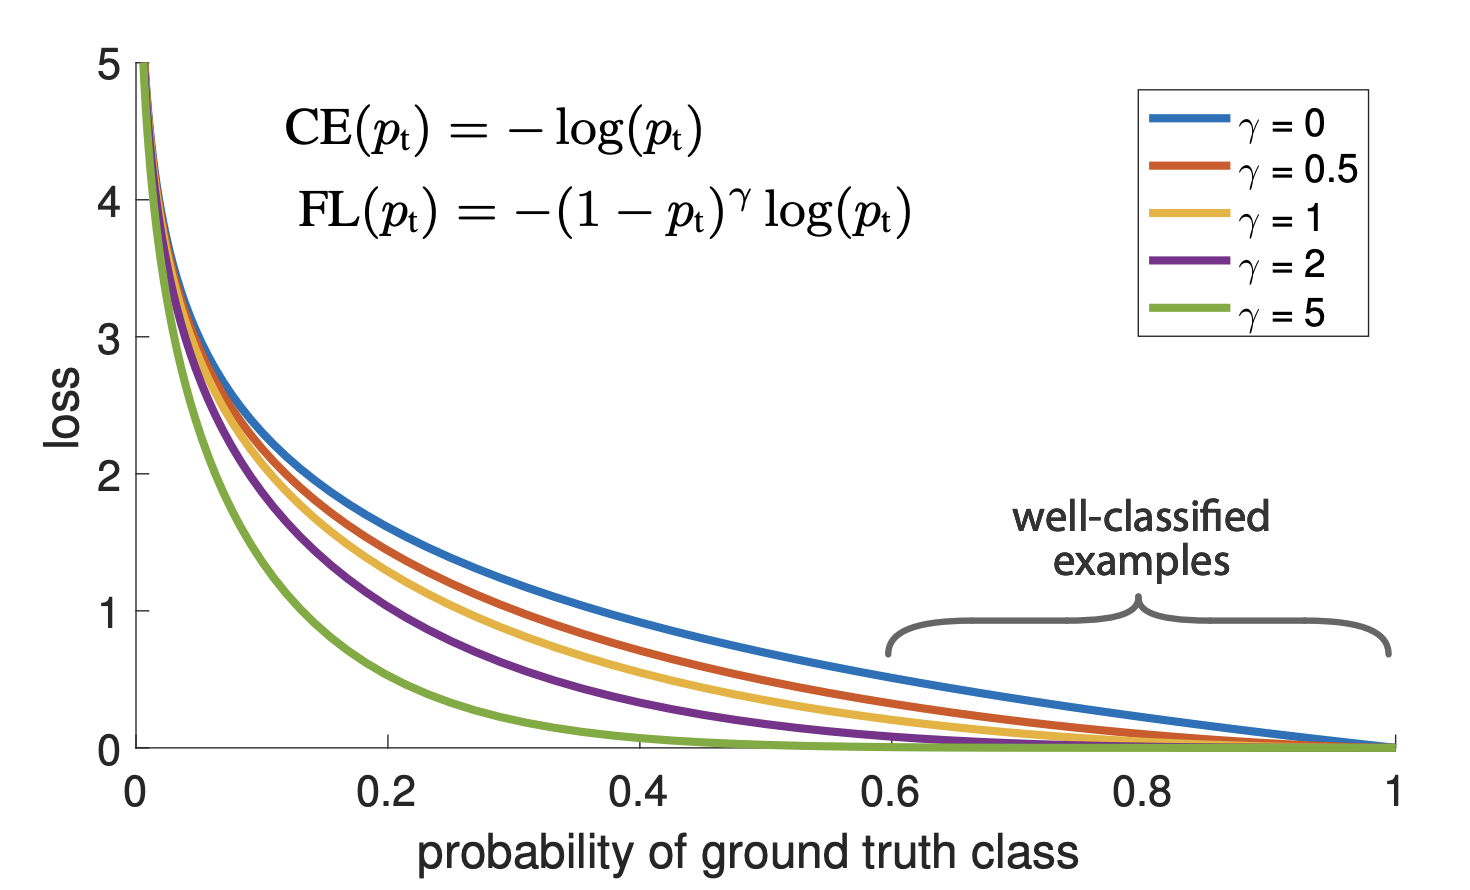
\includegraphics[width=0.7\textwidth]{Illustrations/loss.png}
    \caption{We propose a novel loss we term the Focal Loss that adds a factor}
    \label{fig:my_label}
\end{figure}

\begin{equation}\label{eq_1}
\boxed{Ax=b}
\end{equation}

\begin{equation}
\operatorname{FL}\left(p_{\mathrm{t}}\right)=-\left(1-p_{\mathrm{t}}\right)^\gamma \log \left(p_{\mathrm{t}}\right)
\end{equation}

\begin{equation}\label{eq:CE}
\mathrm{CE}(p, y)= \begin{cases}-\log (p) & \text { if } y=1 \\ -\log (1-p) & \text { otherwise }\end{cases}
\end{equation}